\chapter{Additional Stuff} \label{CHAP:ADD}

\textbf{Memory and Hardware:}

\textbf{SRAM:} Static RAM using flip-flops for feedback loops. Access in 0.5 to 1 nsec.

\textbf{DRAM:} Dynamic RAM, cheaper stores in flip-flop with output capacitance, possibly leaking. Refresh necessary, hence slower.

\textbf{Memory Subsystem Design techniques:}
\begin{itemize}
    \item Memory Interleaving and piepelining
    \item Wide word parallelism
    \item Combination of DRAM and SRAM
\end{itemize}

\textbf{Hardware:} Chip Complexity Scaling (Double components every 2 years), Chip Speeds, Chip I/O (slow increase in pins on chip), Serial I/O (Chip to Chip), Memory Scaling (Access times), Power and Packaging..

\textbf{Network Device Architectures:}

\textbf{Endnodes:} Workstations and so on, Needs external DRAM, speeding up CPU using caches (L1 SRAM, L2 SRAM, uses simple hashes), I/O is memory mapped (NA and Disk look like memory), \textbf{DMA}. Adapters on I/O bus (backwards compatible, i.e., PCI).

\textbf{Routers:} Set of input/output links, needs switching and lookup (consults \textbf{FIB} with LPM), after lookup -> internal switching (I-link to O-link).. and also needs queuing (FIFO if link is congested), Header Validation and Checksums (TTL, IP Checksum, MAC CRC), Protocol processing (SNMP for statistics, ARP synchrionization and more).

\textbf{Virtual Memory:} "Infinite Memory", Mapping of Logical addresses to physical space (can use disk space as memory).

\textbf{Networking:}

\textbf{Protocols:} Ethernet Link layer protocol (MTU ~1500bytes) , uses MAC addresses, Header 14+4 bytes:

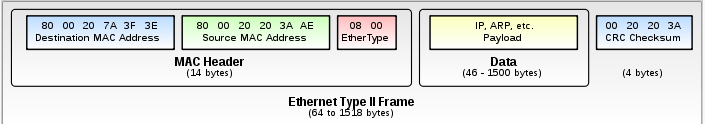
\includegraphics[width=.8\textwidth]{images/chap10/ethernet_header}

\textbf{CRC:} Cyclic redundancy check, basically a hash, can be computed by hardware. Uses polynomial with n-bit order to encode coefficients.

\textbf{IP}: Internet Protocol, used for routing, needs checksum (16 bit, uses TTL, changes every HOP, all 16-bit words in header added up based on ones-complement), Hedaer 20 Bytes + Options:

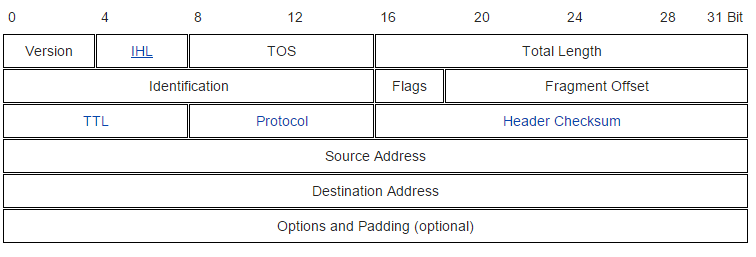
\includegraphics[width=.7\textwidth]{images/chap10/ip_header}

\textbf{TCP:} Transmission Control, Connection-oriented, uses SYN/ACK for state, Checksum (16bit, Uses IP-pseudoheader: SRC/DEST Address, Null-Byte, Val 6 for TCP, TCP Length, pseudoheader not sent), Use slow-start (increase congestion windows with every ACK received, exponential, until slow-start threshold reached or if timeout half threshold and set congestion window to 1), Header 20 - 24 Byte:  

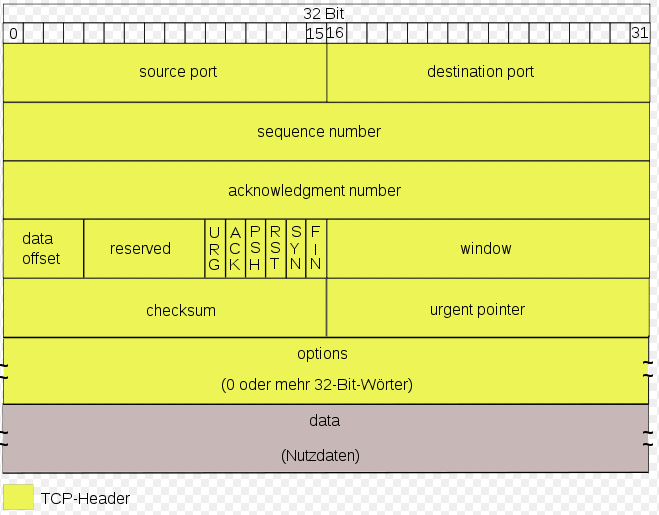
\includegraphics[width=.7\textwidth]{images/chap10/tcp_header}

Minimum Size internet packet: 14+4 + 20 + 20 + 24 = ~60 bytes!